\documentclass[a4paper]{article}

\usepackage[english]{babel}
\usepackage[utf8x]{inputenc}
\usepackage{amsmath}
\usepackage{amsfonts}
\usepackage{url}
\usepackage{graphicx}
\usepackage{comment}
\usepackage{xcolor}
\usepackage[colorinlistoftodos]{todonotes}

\title{CS 5785 -- Applied Machine Learning -- Lec.\ 2}
\author{Profs.\ Nathan Kallus, Cornell Tech\\Scribes: TBD}




\begin{comment}
Brad Wise notes in class - 8/24/17

Bayes Error Rate
- G: Categorical output variable (true instance of class)
	- more general than something like y = {-1, +1}
- G hat = estimate of categorical variable (prediction of class)
	- assumes values in g with K choices (example: if Ivy League, K = 8)
- L: KxK matrix containing loss function - ex for Ivy League Loss: pain you feel at being misclassified
	- L(k, l): price paid for classifying an observation belonging to class Gk as Gl
    - simplest example of loss function: 0 to 1 loss function
    	- simply checks whether right or wrong (if guess wrong, loss is 1. if right, loss is 0)
        
KNN graph example:
15-nearest neighbor
2 classes of training data - Male/Female on 2 dimensions (height and weight)
- compute 15 nearest neighbors to arbitrary point - label as male or female based on majority vote
        
What is KNN (k-nearest neighbor) trying to approximate? 
	- credit fraud example
    
In theory, what is the expected prediction error (EPE)?
	EPE = E[L(G, G hat(x))] 
    additionally, it selects class with highest posterior probability
    	- tells how a point is distributed in space
        
        
KNN vs Bayes Error Rate
- KNN produces cohort of neighbors, works as an approximation
- BER - theoretically, with a Bayes classifier and if you know the underlying Gaussian distribution from your samples, you can get the theoretical optimal curve for your set of data

Footnotes on Bayes Rate
- curse of dimensionality - higher dimensionality will impact the decisions you make with your model
- Bayes rate != Base Rate
	- Bayes Rate - represents theoretically optimal curve if you know underlying distribution
    - Base Rate - 'just go with the prior'
    	- EX: if classifying fruit in a grocery store and picks banana, base rate classifier just guesses 			based on # bananas and total # fruits without looking at other factors like color, texture, etc.
        - if your model doesn't beat the base rate, you need to start over
  
  
  
Linear Regression - in this PDF
- simple learning model
- formulas in PDF
- The Beta, B, in the linear model is a weight related to importance of a variable

- in the linear model, y hat is the predicted result of our classifier and should be scalar
- Additionally, the linear function is represented over p+1 dimensional space, with p being the number of classes in your dataset

Linear regression shape:
- line, like a ramp
- linear classifier
- takes all the data form the classifier
- based on least squares

What is linear regression useful for?
- used for linear separability of data, important for principle components analysis
- simple to use
- fitting a classifier assumes you have found B hat
- y hat = X^T * B hat


How to represent linear regression graphically in 2 Dimensionally:
- A linear regression operates in p+1 space
- Data lives in X,y plane, but because it has a label, the linear function is in p+1 space
- it is treated as a point floating above and below the plane

EX figure 2.1:
Blue = +1
Orange = -1
- this is a quantitative formulation of training data
- graphically something pops in (-1) or out (+1) of the screen
- with an automatic threshold at 0, the way the line tilts predicts our classifier as +1 or -1
	- this will give you a decision boundary
- in our formula, B (knot) represents the offset
	- so adjusting B knot moves our line up or down 

How do we decide values of B hat?
- we must calculate residual sum of squares = RSS(B) formula
- matrix vector notation and design matrix in Section 1.2
	- the design matrix stacks the feature vector X as rows
    
- Solve for B to minimize error and set to 0
	- this will be the "normal equation"
    
Solution to Normal Equations (see section 1.2
- IMPORTANT: X^TX, the design matrix, must be nonsingular (your feature sets should have no duplicates, you should never have copied training examples)
	- if you have duplicate data, you have a deficient matrix, and you can't classify your data
    
Bias Variance Tradeoff
- targets example FIGURE 1, page 4
- a linear regression is a high bias, low variance data set
- LR classifies a lot of data precisely and confidently, but oftentimes, the data classification is wrong

To evaluate Performance of your classifier, it is useful to use different strategies - PERFORMANCE CHARACTERIZATION
EXAMPLES:
- ROC Curve
- precision recall curve
- contingency table (false accept, false reject, etc)
- confusion matrix

EXAMPLES OF CONTINGENCY TABLES
- Mouse example
- if your classifier is perfect and your actual data matches your classifier's predictions, a contingency table would would show a diagonal line

END OF NOTES
\end{comment}




\date{August 28, 2018}

\begin{document}
\maketitle

\section{Linear Regression}
Last lecture we learned about kNN, which is a \emph{lazy learning} or memory-based method, not dependent on a model fit. In lazy learning algorithms, one defers prediction until query time.  In contrast to this, \emph{eager learning} algorithms, work by summarizing the data using a model or function at training time, and then only rely on the summary model at query time.  To illustrate this, we'll look at a method that is somewhat less lazy than kNN, a method that uses a model, albeit a simple one: linear model fit by least squares.

\subsection{The Linear Model}

The model looks like this:
$${\hat Y} = {\hat \beta}_0+\sum_{j=1}^p X_j{\hat \beta}_j$$
with input vector $X=(X_1,X_2,\ldots,X_p)^\top$ and ${\hat \beta}_0$ the intercept or bias.  The hat on symbols indicates a prediction. \\



\begin{comment}
Replace the following with something just beneath. I think this is not really clear. Nicolas

If we like, we can absorb the bias ${\hat \beta}_0$ into the vector of coefficients $X$. $\hat{\beta}$ by adding a constant 1 to the front of $X$.  Then we can write the model very compactly as an inner product:
$$\hat{Y}=X^\top\hat{\beta}$$
\end{comment}

This equation can be shortened by changing the structure of $X$ and concatenating all the $\hat{\beta_i}$ into one vector. The $1$ at the front of this new $X$ absorbs the bias term ${\hat \beta}_0$.

$$ X=(1,X_1,X_2,\ldots,X_p)^\top $$
$$ \hat{\beta} = \begin{pmatrix} \hat{\beta_0} \\ \hat{\beta_1} \\ \vdots \\ \hat{\beta_i} \\ \vdots \\ \hat{\beta_p} \end{pmatrix} $$

These changes of notation enable us to write the following:
$$\hat{Y}=X^\top\hat{\beta}$$

Here we have a single outcome variable, so $\hat Y$ is a scalar, but this can be generalized to multiple outputs $Y_1,\ldots,Y_K$ [HTF \S3.2.4]. \\

Let $f(X)=X^\top\hat{\beta}$ represent some linear function over the $(p+1)$-dim.\ space. We're going to use this function for classification by applying a threshold to $f(X)$.

\begin{comment}
Merv F. (2017-02-01): These "quick notes" were here uncommented when I received the document, however, they appear unnecessary, since both of these topics are cover more fully and in context, later in the notes.

%%%%%%%%%%%%%%%

\emph{Quick Notes:}\\

        We can use this type of regression as a classifier by applying a threshold to the output of the function. For example:

        \[
          \begin{cases}
            \text{``Orange''}     & \quad \text{if } \hat{Y} > 0.8\\
            \text{``Blue''}   & \quad \text{if } \hat{Y} \leq 0.8\\
          \end{cases}
        \]

The gradient of $f$ w.r.t.~$X$ is:

$$ f'(X) = \hat{\beta} $$
\end{comment}

\subsection{Fitting with Least Squares}

How do we fit this model?  In this context, \emph{fit} means ``estimate $\beta$.'' The most popular method for doing this is \emph{least squares}.  In this method, we pick $\beta$ to minimize the \emph{residual sum of squares (RSS)}:\footnote{Also referred to as the \emph{sum of squared residuals (SSR)}.}
$$RSS(\beta)=\sum_{i=1}^N(y_i-X_i^\top\beta)^2$$
In other words, we are looking for the best compromise in $\beta$ over all the data points.

We can write this sum in matrix-vector form as:
$$RSS(\beta) = (y-X\beta)^\top(y-X\beta) = \|y-X\beta\|^2$$
where $X\in\mathbb{R}^{N\times (p+1)}$, a matrix where each row is an input vector, and $y\in\mathbb{R}^N$ is a vector of outputs:
$$X=\left[\begin{array}{ccccc}1&X_1^1&X_2^1&\cdots&X_p^1\\1&X_1^2&X_2^2&\cdots&X_p^2\\\vdots& &\vdots& & \vdots\\1&X_1^N&X_2^N&\cdots&X_p^N\end{array}\right] \qquad y=\left[\begin{array}{c}y^1\\y^2\\\vdots\\y^N\end{array}\right]$$
Here we have $N$ data points and $(p+1)$ dimensions. The matrix $X$ is known as the \emph{design matrix}.

We want to find a $\beta$ vector that will best return the desired values of $y$.  How do we solve for $\beta$?  Optimizing with respect to $\beta$ we have,
\begin{align*}
\nabla_\beta SSR(\beta) &= \nabla_\beta \|y-X\beta\|^2\\
0 &= X^\top(y-X\beta)
\end{align*}
also known as ``the normal equations.''  Provided $X^\top X$ is non singular, we have:
$$\hat{\beta}=(X^\top X)^{-1}X^\top y = X^+y$$
where $X^+=(X^\top X)^{-1}X^\top$ denotes the \emph{pseudoinverse} of $X$.

The fitted value for the $i$th input $x_i$ is:
$$\hat{y}_i=x_i^\top \hat{\beta}$$
which is simply the dot product of the input vector with the fitted coefficients.  Importantly, this applies not just for the input points, it applies for an arbitrary input $x_0$, too!  Thus, the linear model \emph{generalizes} over the plane (space, etc.).  How \emph{well} it generalizes, however, is a different story -- we've made some huge simplifying assumptions here, but it's still noteworthy that we're seeing some actual generalization.

\subsubsection{Why Least Squares? (Optional)}

It is worth considering why least squares is such a popular way of defining a ``best'' fit, because it may appear somewhat arbitrary.  Why not minimize the $l_1$-norm or the $\infty$-norm?  Although we might rule out the $l_1$-norm because it lacks differentiability at the minimum, that criticism doesn't carry over to most other norms.

One of the key features that least squares has is that the error nicely decomposes into recognizable quantities.  Similar to the analysis of expected prediction error (EPE) from the previous lecture, we can analyze the expected error of a given model $f(x)$ as follows,
\begin{align*}
E[(f(X) - Y)^2] &= E_X[E[(f(X) - Y)^2 | X]]\\
&= E_X[f(X)^2 -2 f(X)E[Y|X] + E[Y^2|X]]\\
&= E_X[(f(X) - E[Y|X])^2 + E[Y^2|X] - E[Y|X]^2]\\
&= E_X[(f(X) - E[Y|X])^2] + E[var[Y|X]]\\
&= E_X[f(X) - E[Y|X]]^2 + (E[f(X)^2] - E[f(X)]^2) + E_X[var[Y|X]]\\
&= E_X[f(X) - E[Y|X]]^2 + var[f(X)] + E_X[var[Y|X]]
\end{align*}
The three final terms correspond to the squared \emph{bias} of the model with respect to the data ($E_X[f(x) - E[Y|X]]^2$), the \emph{variance} of the model itself ($var[f(X)]$), and the inherent noise in the data ($E_X[var[Y|X]]$).  Clearly, the choice of model $f(x)$ cannot have any effect on this last component.  Minimizing least squares, therefore, puts squared bias on equal terms with model variance. We will talk more about the notion of a \emph{bias-variance trade-off} later.

\subsection{The ``Linear Classifier''}
\label{sec:linclass}
Let's now bring this back to the classification problem from last lecture, with the response $Y$ coded as 0 for blue and 1 for orange; see HTF Fig.\ 2.1.  We use the convention
$$\hat{G}=\left\{\begin{array}{c}\text{orange, if}\quad\hat{Y}>0.5\\\text{blue, if}\quad\hat{Y}\le 0.5\end{array}\right.$$
The \emph{linear decision boundary} in $\mathbb{R}^2$ is given by $\{x:x^\top\hat{\beta}=0.5\}$ and data points in $\mathbb{R}^2$ get the orange label for $\{x:x^\top\hat{\beta}>0.5\}$

\begin{figure}
\centering
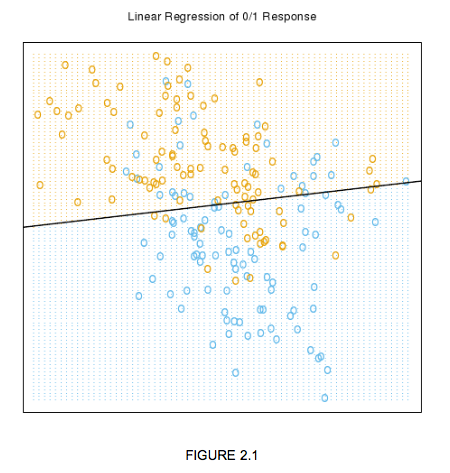
\includegraphics[width=0.75\textwidth]{HTFfig2_1.png}
\end{figure}


How did we do?  We can see the linear model makes a lot of mistakes.  Avoidable?  Yes and no.  One aspect of this approach that should strike us as odd is the binary coding of $Y$ in the face of fitting what amounts to a linear ramp in this case.  Isn't this a strange representation?  We get wildly different contributions to the RSS from pts.\ at varying distance from the decision boundary.

In this sense, linear regression on a $0/1$ response is not very natural.  Soon we'll learn about a more natural way to solve this problem using something called \emph{logistic regression}.

This method is high bias, low variance method. As described by P.~Domingos, ``Bias is a learner’s tendency to consistently learn the same wrong thing. Variance is the tendency to learn random things irrespective of the real signal.'' See Figure \ref{fig:darts} for an illustration of this idea using darts.

\begin{figure}
\centering
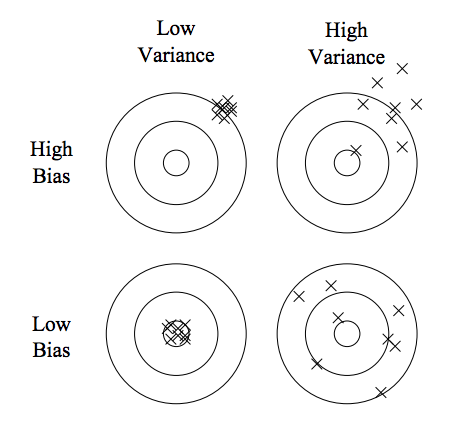
\includegraphics[width=0.5\textwidth]{dartboard.png}
\caption{Bias and Variance in dart throwing. [P.~Domingos 2012]}
\label{fig:darts}
\end{figure}


%Take a dart game for example. If you throw all the darts in the same area anywhere away from the bull eye, you are inaccurate, since you didn't hit the bull eye, but you are consistent, as all the dart impacts are tightly clustered in the same area.

\subsection{Nonlinear Models (Optional)}
The least squares approach is not limited to fitting linear models, but nonlinear models can also be fit by augmenting the feature data with combinations of individual features.  For example, if one had two observed features $z_1$ and $z_2$, a quadratic feature set would take the form

$$ X = \begin{pmatrix} 1 \\ z_1 \\ z_2 \\ z_1^2 \\ z_1 z_2 \\ z_2^2 \end{pmatrix} $$

\subsection{Encoding Categorical Features}
In some problems you'll encounter categorical features encoded as integers, such as \emph{Yale}, \emph{Columbia} and \emph{Cornell} encoded as 0, 1 and 2, respectively.  Multiplying that value by a weight in $\beta$ (as one does in a linear classifier) isn't meaningful.  This is commonly handled by using \emph{one-hot} or \emph{one-of-K} encoding.  For this case, the encoding for these three schools would be the length-3 vectors $[1,0,0]^\top$, $[0,1,0]^\top$ and $[0,0,1]^\top$, respectively.

\section{Performance Evaluation}

Before we dig further into more classification models, we need clarify how we intend to rank or rate the performance of our classifiers. In addition to standardized performance metrics, these measurement involve a bunch of tools used to keep track of what you're doing, how well you're doing and also for debugging purposes. They become our bread and butter for communicating results to others and we need to understand them well.
\subsection{Confusion Matrix}

\begin{figure}
\centering
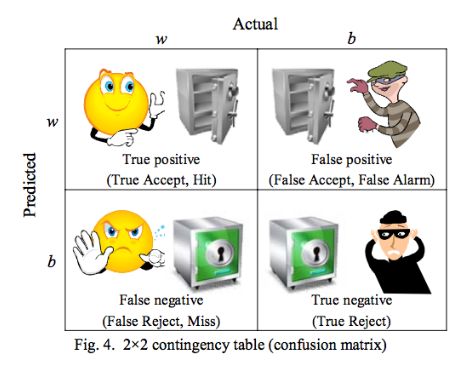
\includegraphics[width=0.75\textwidth]{ChaTappertFig.png}
\caption{\label{contingency_table}Contingency Table (Cha \& Tappert)}
\end{figure}

A confusion matrix, or contingency table, is used to quantify the discrepancies between the ground truth and the ouput of a classifier. In the confusion matrix each column represents the instances in a predicted class, while each row represents the instances in an actual class. The $(i,j)$th entry in the matrix equals the number of observations known to be in class $i$, but predicted by our classifier to be in class $j$. Using this representation, every entry on the diagonal is the number of correctly classified entities of that class. A heavier diagonal implies a more accurate classifier.
Normalizing the matrix, dividing each entry by the sum of all entries (the total number of entities tested) can help calculating the overall error and success rates. The sum of the diagonal of the normalized confusion matrix equals the success rate of the classifier, and the sum of all other cells equals the error rate.

\subsubsection{2$\times$2 Confusion Matrix}
In the case of a \textbf{True-False} classifier there are only two classes and the resulting confusion matrix would is $2\times 2$, a $binary$ confusion matrix; see Figure~\ref{contingency_table}. An example of such a classifier would be an email vs.\ spam classifier; see HTF Table 9.1.

\begin{figure}
\centering
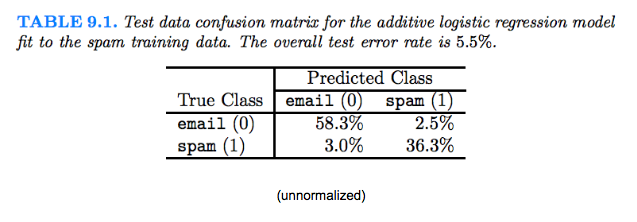
\includegraphics[width=1.0\textwidth]{HTFtable9_1.png}
\label{spam}
\end{figure}

True-positives (TP) and true-negatives (TN) represent correct classifications and False-positives (FP) and false-negatives (FN) represent incorrect classification. FP is also called a \textit{type I} error and FN is also called a \textit{type II} error. The type of error that matters most depends on the problem we are trying to solve. In case of biometrics (e.g., does this fingerprint belong to person $x$?), type I errors are really bad because it means we let the wrong person get past security, while if you have to submit your fingerprint twice to get access it is not that bad. In the case of credit card fraud, in which case the credit provider may be wary of alienating customers, and type II errors become more important. Since the different errors have different significance under different situations, one number is not enough to describe the performance of a classifier. Therefore, be wary if someone tells you ``our system is 99\% accurate!''  Be a stickler: what do they mean by ``accurate?''  Is this a true positive rate?  Perhaps it is simply meaningless.

\subsection{Receiver Operating Characteristic (ROC) Curve}

\begin{figure}
\centering
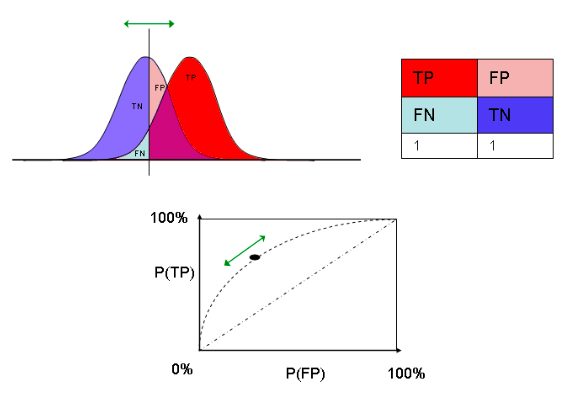
\includegraphics[width=0.75\textwidth]{WikipediaROC.png}
\caption{\label{wikipedia_roc}ROC curve. Top Left: The $x$ axis represents distance or score.  The vertical line represents the classifier threshold setting: scores above the threshold are declared positives. Top Right: 2-class (binary) confusion matrix corresponding to the indicated choice of threshold. Bottom: ROC Curve, with dot representing choice of threshold. Diagonal line represents the ROC curve for random chance.  (Wikipedia)}
\end{figure}

The ROC curve is a graphical means of representing a binary confusion matrix as a function of classifier threshold; see Figure~\ref{wikipedia_roc}. Remember from \S \ref{sec:linclass} that when attempting to fit a linear classifier we get a number representing the score of the classified entity (some function of a distance, for example) and then we \textbf{threshold} it to make a decision. The threshold of the blue/orange problem discussed earlier a depicted in HTF Fig.\ 2.1.\ was $0.5$. Once you commit to a threshold you can create the confusion matrix; every threshold has a corresponding confusion matrix. The ROC curve captures the tradeoff expressed in the confusion matrix as the threshold is swept over a wide range.

The ROC curve plots the \textbf{True Positive Rate} (TPR), or sensitivity, against the \textbf{True Negative Rate} (TNR), or specificity.
$$TPR = \frac{TP}{TP + FN}$$
$$TNR = \frac{TN}{FP + TN}$$

Some version of ROC curves use the \textbf{False Positive Rate} (FPR) instead of TNR. When reading an ROC curve remember to always check which convention is used.
$$FPR = \frac{FP}{FP + TN}$$
\textit{Note: $TNR = 1-FPR$}

\textbf{Accuracy} (ACC) is the number of entities classified correctly over the total number of entities tested. If we denote the total number of positive entities by $P$ and the total number of false entities by $N$ we would get:
$$ACC = \frac{TP+TN}{P+N}$$
In the example from Wikipedia\footnote{\url{http://en.wikipedia.org/wiki/Receiver_operating_characteristic}} (Fig.\ \ref{wikipedia_roc}) $P = N = 100$ creating a \textit{balanced} example.\\

\begin{figure}
\centering
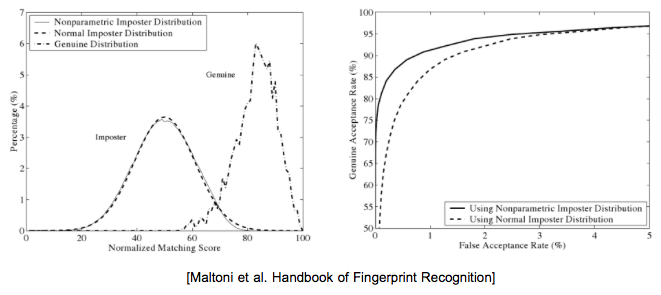
\includegraphics[width=1.0\textwidth]{MaltoniROC.png}
\caption{\label{maltoni_roc}Integrating scores of genuine and impostor pair matches to produce the ROC curve.  As an example, a genuine score would be the similarity between two voiceprints from Alice, while an impostor scores would capture the similarity between a voiceprint form Alice and a voiceprint from Bob.  In general, we expect the distribution of impostor scores to be largely to the left of the genuines, but some overlap is inevitable. (Maltoni et al.)}
\end{figure}

\subsubsection{Area Under the Curve}
A generic metric for comparing the performance of one algorithm to another across all possible thresholds is to compute the Area Under the [ROC] Curve (AUC or AUROC).  This is generic because it summarizes the overall performance, but individual algorithms with lower AUCs could still be more appropriate in certain application contexts.

\subsubsection{ROC Curve Example: Biometric Identification}
Let's look at an example from the field of biometrics (fingerprint recognition, voice recognition, etc.). In this setting we can examine the distribution of \textit{genuine} and \textit{impostor} scores (or distances) arising from comparisons between all possible pairs of \emph{same} and \emph{different} people, respectively.\footnote{Example: Matching two different impressions of the same finger gives us a \emph{genuine} match score. Matching fingerprints from two different people gives us an \emph{impostor} match score.} Figure~\ref{maltoni_roc} demonstrates the matching scores of both \textit{genuine} and \textit{impostor} pairs and the relationships between them. We then generate the ROC curve by sweeping over the range of possible score thresholds, calculating the TPR and FPR at each threshold and plotting these two values against each other.

Suppose we set our threshold so that we obtain a $1\%$ FNR and a $0.01\%$ FPR.  The way to read this is that we incur (or pay the price of) a $1\%$ rejection rate in exchange for a one-in-ten-thousand false positive rate. The latter is the same as the probability of guessing someone's 4 digit PIN.

\subsection{Precision and Recall}
For datasets that are very skewed (not balanced) TP, FP, TN and FN are not good representations of the performance of the algorithms. In such cases we use:
$$Precision = \frac{TP}{TP+FP}$$
$$Recall = \frac{TP}{TP+FN}$$
$$F-Score = \frac{2}{\frac{1}{Precision}+\frac{1}{Recall}}$$
\textit{Note: F-Score is the harmonic mean of Precision and Recall.}

Document retrieval is an example of a problem with a skewed dataset. Imagine you type in a search query and some algorithm computes a similarity score over a set of stored documents. The threshold you sweep here are the number of results presented to the user. In this scenario:
$$Precision = \frac{|\{\text{Relevant Documents}\}\cap\{\text{Retrieved Documents}\}|}{|\{\text{Retrieved Documents}\}|}$$
$$Recall = \frac{|\{\text{Relevant Documents}\}\cap\{\text{Retrieved Documents}\}|}{|\{\text{Relevant Documents}\}|}$$

Precision and Recall can be plotted together too, similar to the ROC curve.
\textit{See Davis \& Goadrich ICML06 to learn more about the connections between ROC curves and precision ancall.}


\end{document}
